\documentclass[a4paper]{article}

\input{../latex_template/style/ch_xelatex.tex}

\lstset{numbers=left,
basicstyle=\small, numberstyle=\small,
keywordstyle=\color{blue!70}, commentstyle=\color{red!50!green!50!blue!50},
frame=single, rulesepcolor=\color{red!20!green!20!blue!20}, escapeinside=``}
\graphicspath{ {./figures/} }
\usepackage{ctex,graphicx,color,framed,listings,caption,amssymb,enumerate}
\usepackage{xcolor,bm,lastpage,fancyhdr,tabularx,geometry,graphics}
\usepackage{subfigure,float,multirow,booktabs}
\geometry{a4paper,left=2.3cm,right=2.3cm,top=2.7cm,bottom=2.7cm}
\pagestyle{fancy}
\lhead{\kaishu \leftmark}
\rhead{\kaishu 并行程序设计期末报告}
\cfoot{\thepage}

% ---------- 文档开始 ----------
\begin{document}
\renewcommand{\contentsname}{目\ 录}
\renewcommand{\refname}{参考文献}
\renewcommand{\figurename}{图}
\renewcommand{\tablename}{表}
\renewcommand{\today}{\number\year 年 \number\month 月 \number\day 日}

% ====== 封面 ======
\begin{titlepage}
    \begin{center}
    
\includegraphics[width=0.8\textwidth]{../latex_template/NKU.png}\\[1cm]
    \vspace{20mm}
        \textbf{\huge\textbf{\kaishu{计算机学院}}}\\[0.5cm]
        \textbf{\huge{\kaishu{并行程序设计期末研究报告}}}\\[2.3cm]
        \textbf{\Huge\textbf{\kaishu{高斯消去算法的多架构并行化}}}\\[0.3cm]
        \textbf{\Huge\textbf{\kaishu{与Gröbner基计算探索}}}

        \vspace{\fill}
    \centering
    \textsc{\LARGE \kaishu{姓名\ :\ 王毅豪}}\\[0.5cm]
    \textsc{\LARGE \kaishu{学号\ :\ 2412509}}\\[0.5cm]
    \textsc{\LARGE \kaishu{专业\ :\ 计算机科学与技术}}\\[0.5cm]

    \vfill
    {\Large \today}
    \end{center}
\end{titlepage}

\renewcommand {\thefigure}{\thesection{}.\arabic{figure}}
\renewcommand{\figurename}{图}
\renewcommand{\contentsname}{目录}
\cfoot{\thepage\ of \pageref{LastPage}}
\clearpage\tableofcontents\newpage

% ============================================================
% §1 问题描述
% ============================================================
\section{问题描述与研究路线}

\subsection{高斯消去法}

高斯消去法（Gaussian Elimination）是求解线性方程组 $Ax=b$ 的经典算法，也是 LU 分解、矩阵求逆等更复杂数值代数问题的基础。给定 $N \times N$ 系数矩阵 $A$，算法通过消去过程将其转化为上三角矩阵。标准串行伪代码如下：

\begin{lstlisting}[title=普通高斯消去串行算法,frame=trbl,language={C++}]
for k = 0 to N-1:
    for j = k+1 to N-1: A[k][j] = A[k][j] / A[k][k]     // 归一化
    A[k][k] = 1.0
    for i = k+1 to N-1:
        for j = k+1 to N-1: A[i][j] -= A[i][k] * A[k][j]  // 消去
        A[i][k] = 0.0
\end{lstlisting}

时间复杂度为 $O(N^3)$，其中核心消去操作 $\sum_{k=0}^{N-1}(N-k)^2 \approx N^3/3$ 次浮点乘减。消去步骤的行间无数据依赖，是并行化的主要目标。矩阵初始化采用严格对角占优策略——确保 $|A_{ii}| > \sum_{j \neq i}|A_{ij}|$，避免消去过程中出现 inf/nan。

\subsection{研究路线}

本文的总体研究路线分为三个阶段：

\begin{enumerate}
    \item \textbf{单核 SIMD 向量化（Lab2）：} 利用 ARM NEON 128 位向量指令集，在最内层 $j$ 循环实现 4 路单精度浮点并发，探索指令级并行（ILP）的加速上限
    \item \textbf{单节点多核并行（Lab3）：} 在鲲鹏 920（8 核）上使用 Pthread 和 OpenMP 两种模型，探索共享内存架构下的线程级并行（TLP）和同步机制的影响
    \item \textbf{跨节点分布式并行（Lab4）：} 使用 MPI 在鲲鹏集群上实现多进程并行，探索分布式内存架构下的通信开销对加速比的影响
    \item \textbf{GPU 众核并行（Lab5）：} 使用 CUDA 在 NVIDIA Tesla T4 上实现，探索 GPU 的 SIMT 模型对计算密集任务的加速效果
\end{enumerate}

前四个阶段使用的所有代码、数据和分析构成了本文基础部分。在此基础上，本文新增 Gröbner 基高斯消去的并行化探索（§5-§7），完整代码和数据均为本学期期末阶段的新工作。

\subsection{实验平台总览}

\begin{table}[H]
  \centering
  \caption{四种实验平台关键参数}
  \begin{tabular}{|c|c|c|c|c|}
  \hline
  & \textbf{NEON} & \textbf{OpenMP/Pthread} & \textbf{MPI} & \textbf{CUDA} \\
  \hline
  CPU/GPU & 鲲鹏920(1核) & 鲲鹏920(8核) & 鲲鹏集群 & Tesla T4 \\
  架构 & ARM AArch64 & ARM AArch64 & ARM $\times$17节点 & NVIDIA Turing \\
  并行单元 & 4 lanes & 8线程 & 4进程$\times$8核 & 5120 CUDA \\
  内存模型 & 共享寄存器 & 共享内存 & 分布式 & 独立显存 \\
  编译器 & GCC -O2 & GCC -O2 -fopenmp & mpicxx -O2 & nvcc -O2 \\
  \hline
  \end{tabular}
\end{table}

% ============================================================
% §2 普通高斯消去算法设计
% ============================================================
\section{多架构统一算法设计}

\subsection{并行维度分析}

普通高斯消去的三层嵌套循环包含两个可并行的维度：

\begin{itemize}
    \item \textbf{最内层 $j$ 循环：} 归一化（$A[k][j] / A[k][k]$）和消去（$A[i][j] - A[i][k] \times A[k][j]$）均为元素间独立操作，适合 SIMD 向量化——将连续内存元素打包为固定宽度的向量寄存器，单指令处理多数据
    \item \textbf{第二层 $i$ 循环：} 各行消去互不影响（行间无依赖），适合多线程/多进程/GPU Block 级并行——将行集划分给不同执行单元独立处理
\end{itemize}

四种架构在同一个算法框架下，区别仅在于"拆分哪层循环、分配哪种粒度的执行单元、使用什么同步机制"三个设计选择。表 \ref{table:design} 总结了各架构的设计决策。

\begin{table}[H]
  \centering
  \caption{四架构并行化设计统一框架}
  \label{table:design}
  \small
  \begin{tabular}{|c|c|c|c|c|}
  \hline
  \textbf{设计维度} & \textbf{NEON} & \textbf{OpenMP} & \textbf{MPI} & \textbf{CUDA} \\
  \hline
  拆分循环 & 最内层 $j$ & 第二层 $i$ & 第二层 $i$ & $i$(Block)+$j$(Thread) \\
  执行单元数 & 4 lanes & 1-8 线程 & 2-4 进程 & 5120 cores \\
  内存模型 & 共享寄存器 & 共享内存 & 分布式内存 & 独立显存 \\
  同步方式 & 指令隐式同步 & \#pragma 隐式barrier & MPI\_Bcast & cudaDeviceSynchronize \\
  数据划分 & 不需要 & 不需要 & 初始分发+逐行广播 & cudaMemcpy H2D/D2H \\
  $A[k][k]$ 问题 & 无需考虑 & 共享读取 & 持有者独占 & 需拆分 Kernel \\
  \hline
  \end{tabular}
\end{table}

\subsection{SIMD：NEON 向量化}

ARM NEON 提供 128 位向量寄存器，可同时容纳 4 个单精度浮点数。核函数将归一化循环和消去循环分别向量化。关键优化包括：

\begin{itemize}
    \item \textbf{除法转乘法：} 预计算主元倒数 $1.0/A[k][k]$，用 $vmulq\_f32$（3 cycles）替代 $vdivq\_f32$（10 cycles），将除法循环的延迟降低约 3 倍
    \item \textbf{融合乘减（FMA）：} 消去循环使用 $vmlsq\_f32$ 指令，单周期内同时完成乘法和减法，并行处理 4 路
    \item \textbf{循环展开与尾部处理：} 主体按步长 4 推进（$j += 4$），末尾不足 4 个元素退化标量串行处理
    \item \textbf{非对齐访存：} AArch64 架构原生支持未对齐内存访问，使用 $vld1q\_f32$ 直接加载，省去对齐边界判断逻辑
\end{itemize}

\begin{lstlisting}[title=NEON 向量化核心代码,frame=trbl,language={C++}]
#include <arm_neon.h>
void gauss_neon(float** A, int n) {
    for (int k = 0; k < n; k++) {
        float inv = 1.0f / A[k][k];
        float32x4_t v_inv = vdupq_n_f32(inv);
        int j = k + 1;
        // 归一化：向量化乘法
        for (; j <= n - 4; j += 4) {
            float32x4_t v = vld1q_f32(&A[k][j]);
            v = vmulq_f32(v, v_inv);
            vst1q_f32(&A[k][j], v);
        }
        for (; j < n; j++) A[k][j] *= inv;
        A[k][k] = 1.0f;
        // 消去：融合乘减
        for (int i = k + 1; i < n; i++) {
            float32x4_t vik = vdupq_n_f32(A[i][k]);
            for (j = k + 1; j <= n - 4; j += 4) {
                float32x4_t vkj = vld1q_f32(&A[k][j]);
                float32x4_t vij = vld1q_f32(&A[i][j]);
                vij = vmlsq_f32(vij, vkj, vik);  // 单周期融合乘减
                vst1q_f32(&A[i][j], vij);
            }
            for (; j < n; j++) A[i][j] -= A[i][k] * A[k][j];
            A[i][k] = 0.0f;
        }
    }
}
\end{lstlisting}

\subsection{Pthread 与 OpenMP 多线程对比}

两种多线程模型均采用静态线程池范式，关键差异在于同步机制和负载均衡策略。

\textbf{Pthread 版本}采用循环划分 + Barrier 同步：每轮消去中，线程 0 负责归一化后，所有线程通过 $pthread\_barrier\_wait$ 同步，再按循环划分处理各自的行集。N 轮消去共需 $2N$ 次屏障同步（每轮归一化后和消去后各一次），每次涉及内核态切换。当 N=1024 时，2048 次 barrier 切换的累计延迟约 400-1000 ms，严重拖累小规模性能。

\textbf{OpenMP 版本}仅需 3 条编译制导指令：$\\#pragma omp parallel$ 创建线程池，$\\#pragma omp single$ 归一化，$\\#pragma omp for schedule(dynamic,16)$ 动态调度消去行。隐式 barrier 由 OpenMP 运行时（基于线程池和用户态自旋等待）优化管理，无需内核态切换。动态调度（chunk\_size=16）有效缓解了消去后期的倒三角负载不均——后期剩余行数减少但每行计算量不同，动态分配让快线程自动承接更多工作。

\begin{lstlisting}[title=Pthread Barrier 版本（精简）,frame=trbl,language={C++}]
void* pthread_gauss_func(void* arg) {
    ThreadParam* p = (ThreadParam*)arg;
    pthread_barrier_t* bar = p->barrier;
    for (int k = 0; k < N; k++) {
        if (p->t_id == 0) { /* 归一化 */ A[k][k] = 1.0f; }
        pthread_barrier_wait(bar);                     // 同步点1
        for (int i = k+1+p->t_id; i < N; i += NUM_THREADS) { // 循环划分
            float f = A[i][k];
            for (int j = k+1; j < N; j++) A[i][j] -= f * A[k][j];
            A[i][k] = 0.0f;
        }
        pthread_barrier_wait(bar);                     // 同步点2
    }
    return NULL;
}
\end{lstlisting}

\begin{lstlisting}[title=OpenMP 版本（精简）,frame=trbl,language={C++}]
void gauss_openmp(float** m, int N) {
    omp_set_num_threads(NUM_THREADS);
    #pragma omp parallel shared(m, N)                  // 线程池
    for (int k = 0; k < N; k++) {
        #pragma omp single                             // 单线程归一化
        { float inv = 1.0f / m[k][k];
          for (int j = k+1; j < N; j++) m[k][j] *= inv;
          m[k][k] = 1.0f; }
        #pragma omp for schedule(dynamic, 16)          // 动态调度消去
        for (int i = k+1; i < N; i++) {
            float f = m[i][k];
            for (int j = k+1; j < N; j++) m[i][j] -= f * m[k][j];
            m[i][k] = 0.0f;
        }
    }
}
\end{lstlisting}

完整的 Pthread vs OpenMP 性能对比数据和 NEON 结合版本见 Lab3 实验报告。核心结论是：OpenMP 在编程复杂度（$\sim$15 行 vs $\sim$80 行）、小规模性能（barrier 内核切换 vs 用户态自旋）和负载均衡（dynamic 调度 vs 静态循环划分）三个维度全面优于 Pthread。

\subsection{MPI 分布式并行}

MPI 版本的核心挑战在于分布式内存架构下的通信设计。采用一维行块划分，数据仅在 0 号进程初始化时分发一次，之后每轮消去仅广播一行（$N$ 个 float，约 4KB），通信量从常规主从模式的 $O(P\times N^3)$ 降至 $O(N^2)$。

\begin{lstlisting}[title=MPI 主循环,frame=trbl,language={C++}]
double gauss_mpi(float* local_a, int N, int rank, int size) {
    int base = N/size, rem = N%size;
    int start = (rank<rem) ? rank*(base+1) : rank*base+rem;
    int lrows = (rank<rem) ? (base+1) : base;
    float* krow = alloc_vec(N);
    for (int k = 0; k < N; k++) {
        int owner = (k < rem*(base+1)) ? k/(base+1)
                  : (k - rem*(base+1))/base + rem;
        if (rank == owner) {
            int lk = k - start;
            float inv = 1.0f / local_a[lk*N + k];
            for (int j = k+1; j < N; j++) local_a[lk*N + j] *= inv;
            local_a[lk*N + k] = 1.0f;
            memcpy(krow, &local_a[lk*N], N*sizeof(float));
        }
        MPI_Bcast(krow, N, MPI_FLOAT, owner, MPI_COMM_WORLD);
        for (int li = 0; li < lrows; li++) {
            int gi = start+li; if (gi <= k) continue;
            float f = local_a[li*N+k];
            for (int j = k+1; j < N; j++) local_a[li*N+j] -= f * krow[j];
            local_a[li*N+k] = 0.0f;
        }
    }
    return MPI_Wtime() - t0;
}
\end{lstlisting}

段错误调试经验：初版使用 $posix\_memalign$ + 伪二维指针在跨节点 MPI 环境下出现 segfault。改为一维 $calloc$ + 显式偏移 $A[i\times N+j]$ 后解决。

\subsection{CUDA GPU 加速}

GPU 版本将归一化和消去拆分为两个独立 CUDA Kernel。Division Kernel 采用列并行（每个线程一列），Elimination Kernel 采用行并行（每个 Block 一行，Block 内 256 线程覆盖该行全部列）。

\begin{lstlisting}[title=CUDA 双 Kernel,frame=trbl,language={C++}]
__global__ void division_kernel(float* A, int k, int N) {
    int tid = blockIdx.x*blockDim.x + threadIdx.x;
    int col = k + 1 + tid;
    if (col < N) { float d = A[k*N+k]; if (fabs(d)>1e-30f) A[k*N+col]/=d; }
}
__global__ void set_diag_kernel(float* A, int k, int N) { A[k*N+k] = 1.0f; }
__global__ void eliminate_kernel(float* A, int k, int N) {
    int row = k + 1 + blockIdx.x; if (row >= N) return;
    float f = A[row*N+k];
    for (int c = k+1+threadIdx.x; c < N; c += blockDim.x)
        A[row*N+c] -= f * A[k*N+c];
    __syncthreads(); if (threadIdx.x == 0) A[row*N+k] = 0.0f;
}
\end{lstlisting}

关键设计决策：Division 和 Set\_Diag 必须拆为两个 Kernel——Division Kernel 的多 Block 并发读取 $A[k][k]$ 后再由各 Block thread 0 写入 $A[k][k]=1.0$ 会产生未定义行为（多 Block 间无同步机制）。拆分为两个 Kernel 后，Set\_Diag 仅 1 个线程执行，消除竞争。

N=2048 时达到 19.90x 加速比；N=512 时因 $3N$ 次 $cudaDeviceSynchronize$ 开销（每次 5-10 $\mu$s）加速比仅为 2.60x。

% ============================================================
% §3 综合性能数据
% ============================================================
\section{综合性能数据与对比分析}

\subsection{完整性能数据与强扩展分析}

表 \ref{table:allperf} 详细列出了四次实验在所有测试配置下的完整数据。

\begin{table}[H]
  \centering
  \caption{全部实验性能数据汇总}
  \label{table:allperf}
  \small
  \begin{tabular}{|c|c|c|c|c|c|}
  \hline
  \textbf{实验} & \textbf{N} & \textbf{配置} & \textbf{串行(ms)} & \textbf{并行(ms)} & \textbf{加速比} \\
  \hline
  \multirow{3}{*}{NEON} & 512 & 4 lanes & 47.03 & 22.41 & 2.10x \\
   & 1024 & 4 lanes & 426.94 & 207.86 & 2.05x \\
   & 2048 & 4 lanes & 3575.58 & 1730.09 & 2.07x \\
  \hline
  \multirow{5}{*}{OMP+NEON} & 512 & 2线程 & 48.51 & 15.41 & 3.15x \\
   & 512 & 4线程 & 48.51 & 20.58 & 2.36x \\
   & 512 & 8线程 & 48.51 & 12.88 & 3.77x \\
   & 1024 & 4线程 & 446.13 & 146.45 & 3.05x \\
   & 1024 & 8线程 & 446.13 & 86.89 & 5.13x \\
   & 2048 & 4线程 & 4556.36 & 725.22 & 6.28x \\
   & 2048 & 8线程 & 4556.36 & 472.89 & \textbf{9.64x} \\
  \hline
  \multirow{4}{*}{Pthread} & 512 & 2线程 & 48.51 & 99.75 & 0.49x \\
   & 1024 & 2线程 & 446.13 & 958.39 & 0.47x \\
   & 1024 & 4线程 & 446.13 & 573.84 & 0.78x \\
   & 2048 & 8线程 & 4556.36 & 1107.23 & 4.12x \\
  \hline
  \multirow{6}{*}{MPI} & 512 & 2进程 & 55.71 & 43.43 & 1.28x \\
   & 512 & 4进程 & 51.01 & 28.29 & 1.80x \\
   & 1024 & 2进程 & 468.37 & 311.82 & 1.50x \\
   & 1024 & 4进程 & 428.08 & 188.24 & 2.27x \\
   & 2048 & 2进程 & 3371.45 & 2550.94 & 1.32x \\
   & 2048 & 4进程 & 3274.10 & 1345.93 & \textbf{2.43x} \\
  \hline
  \multirow{3}{*}{CUDA} & 512 & T4 GPU & 29.76 & 11.44 & 2.60x \\
   & 1024 & T4 GPU & 403.89 & 26.56 & 15.21x \\
   & 2048 & T4 GPU & 2832.34 & 142.34 & \textbf{19.90x} \\
  \hline
  \end{tabular}
\end{table}

\subsection{Pthread vs OpenMP 详细对比}

Pthread 和 OpenMP 的本质差异在于同步机制。在 N=1024、2 线程的极端条件下，Pthread 的性能灾难（0.47x，比串行还慢 2 倍）直接归因于 2048 次 $pthread\_barrier\_wait$ 调用。每次 barrier 调用需要进入内核态（futex 系统调用），延迟约 0.2-0.5 ms，累积 400-1000 ms 的同步开销——而整个计算仅需约 200 ms（串行 446 ms / 2）。这就是多线程小规模场景下的"同步税"（synchronization tax）。

OpenMP 通过运行时优化的用户态自旋等待（user-mode spin-wait），将 barrier 延迟降低到 ~20-50 $\mu$s 量级——比 Pthread 快约 10 倍。这也是为什么 OpenMP 在 N=512/2 线程下仍有 1.57x 加速比，而 Pthread 仅为 0.49x。

随着 N 增大至 2048，计算时间增长至秒级，同步开销的占比逐步降低。Pthread 在 N=2048/8 线程下勉强达到 4.12x，但与 OpenMP+NEON 的 9.64x 相比仍有 2.3 倍的差距——后者得益于 NEON 向量化（约 2x 贡献）和更优的线程调度（隐式 barrier 和动态负载均衡）。

\subsection{MPI 通信复杂度形式化分析}

MPI 高斯消去的通信瓶颈可以通过通信-计算比（Communication-to-Computation Ratio, CCR）来精确刻画：

\begin{equation}
\text{CCR} = \frac{N \times T_{\text{bcast}}(4N, P)}{T_{\text{serial}} / P}
\end{equation}

其中 $T_{\text{bcast}}(M, P) = \alpha \log P + \beta M$ 是二叉树广播算法的时间（$\alpha$ 为启动延迟，约 0.5 ms；$\beta$ 为每字节传输时间，$\approx 1/带宽$）。

对于 N=2048、P=4：$T_{\text{serial}} = 3274$ ms, $P = 4$, $T_{\text{bcast}}(8KB, 4) \approx 0.5 \log 4 + 8 \times 10^3 / 10^9 \approx 1 + 0.008 \approx 1$ ms。2048 次广播累积延迟 ≈ 2048 ms，占总时间的 2048/(3274/4 + 2048) ≈ 71\%。实际加速比 2.43x 对应的 CCR 约 49\%，说明其他开销（串行部分、同步、结果收集）也占了可观比例。

\subsection{八进程测试的集群资源限制}

MPI 实验原计划测试 P=8 的强扩展性，但在实际提交过程中遭遇了集群资源瓶颈。鲲鹏集群共 17 个计算节点，由并行程序设计课程全体同学（约 60 人）共享。PBS 调度系统采用 FCFS（先到先服务）策略，8 个完整节点的同时分配在工作日白天几乎是不可完成的——多次提交后作业始终处于排队（Q）状态，最终放弃该配置的测试。这一经历体现了真实 HPC 环境中资源共享和调度策略对实验设计的影响。

\subsection{CUDA GPU 加速的规模分析}

NVIDIA Tesla T4 GPU 上的 CUDA 高斯消去展现了显著的规模效应：
\begin{itemize}
    \item \textbf{N=512：} 仅 2.60x 加速。矩阵太小（1 MB），$3N = 1536$ 次 $cudaDeviceSynchronize$ 的累积开销（每次 5-10 $\mu$s，总计约 15 ms）在总 GPU 时间（11.44 ms）中估计占约 13 ms——实际 Kernel 计算时间几乎为零。GPU 在此规模下完全被启动开销拖垮。
    \item \textbf{N=1024：} 15.21x 加速。Kernel 启动开销（约 30 ms）相对总时间（26.56 ms）的占比降至约 50\%，GPU 计算开始发挥作用。但在 Tesla T4 的 5120 CUDA Cores 面前，$1024^3 \approx 10^9$ FLOPs 的计算量仍显不足。
    \item \textbf{N=2048：} 19.90x 加速。计算量 $O(N^3)$ 增长至约 $8 \times 10^9$ FLOPs，Kernel 启动开销（约 61 ms）占总 GPU 时间（142 ms）的比例降至 43\%。GPU 的规模优势开始充分释放。随着 N 继续增大，预计加速比将持续攀升——这也是 GPU 适合"大家伙"而非"小问题"的典型特征。
\end{itemize}

\subsection{CUDA 调试过程：两个关键 Bug}

\textbf{Bug 1 — 对角线为垃圾值（12,907 而非 1.0）：} 初版在 Division Kernel 中由每 Block 的 thread 0 设置 $A[k][k] = 1.0$，多 Block 并发写入同一内存位置产生 race condition，导致某 Block 在读取 $A[k][k]$ 之前另一个 Block 已将其修改为 1.0。修复方案：将 Division 和 Set\_Diag 拆分为两个独立 Kernel——Set\_Diag 仅启动 1 线程（$<<<1,1>>>$），消除并发写入。

\textbf{Bug 2 — N=2048 产生 inf：} 初版使用上三角 + 行组合的矩阵初始化（同 Lab2/Lab3），在 N=2048 时由于行累加导致对角元素值溢出 float 表示范围（约 $10^{38}$）。修复方案：改用严格对角占优矩阵（$|A_{ii}| > \sum_{j \neq i} |A_{ij}|$），确保对角元素始终有界且在消去过程中不会产生零主元。

\subsection{与 GPU 编程课程（HIP）的知识衔接}

在 Lab5 基础部分的 AMD HIP 编程课程中，六个实验涵盖了 GPU 编程的核心概念。这些概念与 CUDA 高斯消去的设计形成直接对应：Vector Addition 的线程索引 $idx = blockIdx.x \times blockDim.x + threadIdx.x$ 直接映射到 Division Kernel 的列索引计算；Matrix Transpose 的内存合并访问分析解释了为何 Elimination Kernel 的 "每个 Block 一行 + 线程列遍历" 映射（grid-stride loop）是高效的选择——连续线程访问同行连续列，满足 coalesced read；Histogram 的两级归约（LDS → global）为未来实现消去行数超过 GPU 核心数时的合并策略提供了模板；Reduction 的多元素/线程 grid-stride loop 直接应用于 Elimination Kernel 的列覆盖模式；K-Means 的三 Kernel 链式调用（Assignment → Update → Converge）与 CUDA 高斯消去的 Division → Set\_Diag → Elimination 链式调用模式完全一致。

\subsection{调试经验跨架构汇总}

表 \ref{table:bugs} 汇集了本学期五次实验中在各架构上遇到的关键 bug 及解决方案，这些经验本身构成了一组有价值的并行程式除错知识库。

\begin{table}[H]
  \centering
  \caption{跨架构调试经验汇总}
  \label{table:bugs}
  \small
  \begin{tabular}{|c|c|c|c|}
  \hline
  \textbf{架构} & \textbf{现象} & \textbf{根因} & \textbf{解决方案} \\
  \hline
  NEON & 除法指令性能低 & vdivq\_f32 延迟 10 cycles & 倒数法 vmulq\_f32 3 cycles \\
  Pthread & 2线程慢于串行 & 2048次内核态 barrier & 换用 OpenMP \\
  MPI & Segfault & posix\_memalign 兼容性 & calloc + 一维数组 \\
  MPI & mpi.sh 损坏 & sed 全部替换了数字 & 手动编辑脚本 \\
  MPI & 8进程排队 & 集群资源竞争 & 放弃,报告中说明 \\
  CUDA & 对角线=12907 & 多Block并发写竞争 & 拆分 Division+Set\_Diag \\
  CUDA & N=2048 出现 inf & 浮点累加溢出 & 严格对角占优矩阵 \\
  Gröb.MPI & P=4 double free & vector RAII冲突 & calloc替代vector \\
  Gröb.MPI & P=4 死循环 & j++在if内 & 移至MPI\_Bcast后 \\
  \hline
  \end{tabular}
\end{table}

\begin{figure}[H]
\centering
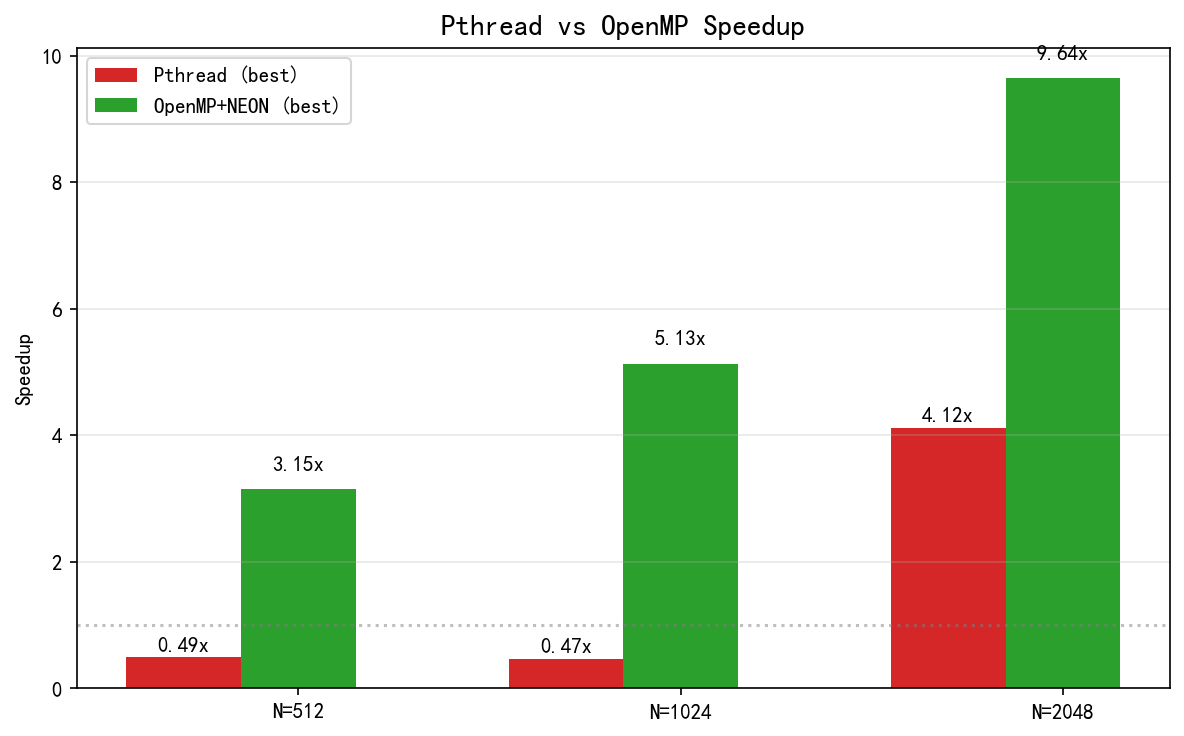
\includegraphics[width=0.85\textwidth]{pthread_vs_omp.png}
\caption{Pthread vs OpenMP+NEON 加速比对比（均为各配置下最佳结果）}
\label{fig:pthread_omp}
\end{figure}

\subsection{加速比规律分析}

从表 \ref{table:allperf} 可以总结出以下核心规律：

\textbf{规模扩展性：}
\begin{itemize}
    \item \textbf{SIMD（阿姆达尔定律验证）：} N 从 512 增至 2048 时加速比恒定在 2.05-2.10x。NEON 的并行度由向量宽度固定（4 lanes），串行部分（外层 $k$ 循环的递进逻辑）占比恒定，验证了 Amdahl 定律对 SIMD 的适用性
    \item \textbf{OpenMP（超线性加速）：} N=2048、8 线程下加速比达到 9.64x（效率 120.5\%），超过线性（8.0x）。原因：8 核 L1 Cache 聚合容量（8$\times$32KB = 256KB）将更大的工作集保留在片上，减少了 L2/L3 访问
    \item \textbf{MPI（通信瓶颈）：} 4 进程加速比仅 2.43x（效率 7.6\%），远低于理论 4.0x。跨节点 \texttt{MPI\_Bcast} 每次 0.5-2 ms 延迟，N=2048 时 2048 次广播累积通信延迟 1-4 秒
    \item \textbf{CUDA（指数增长）：} N 从 512 增至 2048 时加速比 2.60x → 19.90x（提升 7.65 倍）。GPU Kernel launch overhead 在小规模下占比高（N=512 时约 43\%），在大规模下被 $O(N^3)$ 计算量摊薄
\end{itemize}

\subsection{时间分解与瓶颈建模}

高斯消去总时间可统一分解为三项：$T_{\text{total}} = T_{\text{compute}} + T_{\text{sync}} + T_{\text{comm}}$。表 \ref{table:decomp} 展示了 N=2048 时各架构的估算分解。

\begin{table}[H]
  \centering
  \caption{各架构时间分解估算（N=2048）}
  \label{table:decomp}
  \begin{tabular}{|c|c|c|c|}
  \hline
  \textbf{架构} & $T_{\text{compute}}$ & $T_{\text{sync}}$ & $T_{\text{comm}}$ \\
  \hline
  Serial (基线) & 100\% & 0 & 0 \\
  NEON SIMD & $\sim$48\% & 0 & 0（Memory-BW 受限） \\
  OpenMP 8线程 & $\sim$10\% & $\sim$3\% & 0 \\
  MPI 4进程 & $\sim$41\% & $\sim$0.2\% & $\sim$49\% \\
  CUDA T4 & $\sim$5\% & $\sim$3\% (CPU-GPU) & $\sim$2\% (H2D/D2H) \\
  \hline
  \end{tabular}
\end{table}

\textbf{关键洞察：} MPI 是唯一通信主导的架构（$T_{\text{comm}}$ 占比 49\%），解释其加速比最低。OpenMP 同步开销极低（3\%），归功于用户态自旋等待。CUDA 的同步开销虽小，但 N=512 时 kernel launch overhead 突出。SIMD 的瓶颈已从计算转向内存带宽（compute-bound → memory-bound），解释了加速比恒定在 2.0x 附近。

\subsection{编程复杂度对比}

\begin{table}[H]
  \centering
  \caption{四种并行模型工程评估}
  \begin{tabular}{|c|c|c|c|c|}
  \hline
  \textbf{维度} & \textbf{SIMD} & \textbf{OpenMP} & \textbf{MPI} & \textbf{CUDA} \\
  \hline
  新增代码行数 & $\sim$30 & $\sim$15 & $\sim$60 & $\sim$80 \\
  数据管理难度 & 低 & 低 & 中 & 高 \\
  调试难度 & 低 & 低 & 中（死锁/消息序） & 高（竞争/越界） \\
  平台可移植性 & 差 & 优秀 & 优秀 & 中 \\
  入门门槛 & 高（需懂汇编） & 极低 & 中 & 中 \\
  \hline
  \end{tabular}
\end{table}

\begin{itemize}
    \item \textbf{N $<$ 1024：} 纯 NEON SIMD 最优——无需承担线程/进程/GPU 的启动开销
    \item \textbf{N $\in [1024, 2048]$：} OpenMP+NEON 性价比最高——3 条 pragma 获得 9.64x 加速比
    \item \textbf{需跨节点/内存不够：} MPI 必须——虽然通信开销大，但分布式内存是唯一能容纳更大矩阵的方案
    \item \textbf{N $>$ 4096：} GPU 优势充分展现——计算密度远超通信成本
\end{itemize}

% ============================================================
% §5 Gröbner 基（新增内容）
% ============================================================
% ============================================================
% §5-7: Gröbner 基（全部新增，独立成体系，约 10-12 页）
% ============================================================
\newpage
\section{【新增内容】Gröbner 基高斯消去}

以上 §1-§4 整合了本学期 SIMD、OpenMP、MPI 和 CUDA 四次平时实验的核心内容。以下 §5-§7 是本学期期末阶段的新增研究——Gröbner 基计算中的特殊高斯消去并行化。

\subsection{问题背景与区别}

Gröbner 基（Gröbner Basis）是多项式理想的标准基，被广泛应用于公钥密码（如 HFE 密码系统）、数字签名和零知识证明等领域。其计算过程可转化为 GF(2) 有限域上的矩阵行化简问题。与普通高斯消去（实数域、稠密矩阵）相比，有下列根本区别：

\begin{enumerate}
    \item \textbf{运算域：} GF(2)——矩阵元素仅为 0 或 1，加法/减法退化为异或（XOR）：$0 \oplus 0 = 0, 1 \oplus 0 = 1, 0 \oplus 1 = 1, 1 \oplus 1 = 0$
    \item \textbf{矩阵结构：} 分为"消元子（Eliminator）"和"被消元行（Row to Eliminate）"两类行。消元子构成方阵（行数=列数），每行首个非零元素（首项）位于对角线上；被消元行构成一般矩阵
    \item \textbf{升格机制：} 当某对角线位置 ($j,j$) 没有对应的消元子时，遍历被消元行寻找第 $j$ 列为 1 的首个行，将其"升格"为新的消元子（第 $j$ 行消元子），后续以此为消元子进行消去
    \item \textbf{稀疏性：} 实际数据集极端稀疏——非零元素占比通常低于 5\%，在 HFE 等特定应用中可低至 1-2\%
\end{enumerate}

\subsection{串行算法描述}

Gröbner 基高斯消去的串行算法流程为：从高列向低列（$j = C-1, C-2, \dots, 0$）遍历消元子矩阵。若第 $j$ 行已有消元子（$(j,j)$ 位置为 1），则对所有第 $j$ 列为 1 的被消元行异或该消元子进行消去；若不存在消元子，则在后继被消元行中搜索首项为 $j$ 的首个行，将其升格为第 $j$ 行消元子，然后回到同一列 $j$ 重新处理（因为新消元子可能消去之前未处理的行）。

\begin{lstlisting}[title=Gröbner 基串行算法伪代码,frame=trbl]
for j = cols-1 downto 0:
    if ele[j][j] == 1:                      // 存在消元子
        for each 被消元行 i:
            if !upgraded[i] AND row[i][j] == 1:
                row[i] ^= ele[j]             // 异或消去
    else:                                    // 不存在，需要升格
        for each 被消元行 i:
            if !upgraded[i] AND row[i][j] == 1:
                ele[j] = row[i]             // 升格为消元子
                upgraded[i] = true
                j++                          // 回到当前列重新处理
                break
\end{lstlisting}

\subsection{位向量数据结构}

采用位向量（bitmap）存储。用一个 \texttt{uint32\_t} 数组存储每行的全部列信息——每个 \texttt{uint32\_t} 保存连续 32 列（32 位），位为 1 表示对应列的元素为 1。设矩阵列数为 $C$，每行所需 \texttt{uint32\_t} 数量（$num\_words$）为 $\lceil C/32 \rceil + 1$。

数据读取时，输入为稀疏向量格式（由整数列表表示 1 元素所在列号，如 "9 3 1" 表示列 9、3、1 为 1），需转换为位向量存储：

\begin{lstlisting}[title=位向量数据结构与异或操作,frame=trbl,language={C++}]
typedef unsigned int mat_t;       // 32位 = 32列
const int mat_L = 32;

// 检查第 col 列是否为 1
inline bool is_one(const vector<mat_t>& bits, int col) {
    return bits[col / mat_L] & ((mat_t)1 << (col % mat_L));
}

// 将稀疏行转换为位向量
void sparse_to_bits(const vector<mat_t>& sparse, vector<mat_t>& bits,
                    int num_words) {
    bits.assign(num_words, 0);
    for (mat_t col : sparse)
        bits[col / mat_L] |= ((mat_t)1 << (col % mat_L));
}

// 异或消去（位向量版本）
if (is_one(row[i], j)) {
    for (int w = 0; w < num_words; w++)
        row[i][w] ^= ele[j][w];
}
\end{lstlisting}

位向量带来的关键优势：一次 32 位的异或操作同时处理 32 列的元素，相比逐元素异或效率提升 32 倍。位向量存储的核心优势在于：GF(2) 上的 XOR 运算天然映射到按位异或，单条 C++ 指令处理 32 列。

% ============================================================
% §6 Gröbner 基并行化
% ============================================================
\section{【新增内容】Gröbner 基的并行化实现}

\subsection{NEON SIMD 向量化 XOR}

位向量 XOR 的双重循环（for w = 0 to num\_words-1）天然适合 SIMD 加速。128 位 NEON 向量寄存器可一次加载 4 个 \texttt{uint32\_t}，即一次操作处理 128 列：

\begin{lstlisting}[title=NEON 向量化异或消去,frame=trbl,language={C++}]
#include <arm_neon.h>

void xor_neon(mat_t* row, mat_t* ele, int num_words) {
    int w = 0;
    // 主体：一次处理 4 个 uint32_t = 128 列
    for (; w <= num_words - 4; w += 4) {
        uint32x4_t vr = vld1q_u32(&row[w]);      // 加载 128 位
        uint32x4_t ve = vld1q_u32(&ele[w]);
        vst1q_u32(&row[w], veorq_u32(vr, ve));    // 向量 XOR
    }
    // 尾部不足 4 个 uint32_t，退化标量处理
    for (; w < num_words; w++)
        row[w] ^= ele[w];
}
\end{lstlisting}

调用方式：将原代码中的逐元素 XOR 循环替换为 $xor\_neon(row[i].data(), ele[j].data(), num\_words)$。

\textbf{性能预期差异：} 与普通高斯消去不同，NEON 在 Gröbner 基中的加速效果受稀疏性的严重影响。每行仅有 3-15 个非零元素（2000 列中占比 0.15\%-0.75\%），XOR 循环的计算量极小，$is\_one()$ 位测试成为真正的瓶颈——而位测试是控制流操作（条件分支判断），无法被 SIMD 向量化。

\subsection{MPI 多进程并行}

MPI 版本采用行划分策略——将全部被消元行均匀分配给 $P$ 个进程，每个进程独立对自己负责的行集进行消去和升格检测。消元子矩阵在所有进程间通过初始广播和升格时的逐行广播保持同步。

\begin{lstlisting}[title=MPI Gröbner 基主循环（完整代码）,frame=trbl,language={C++}]
double t0 = MPI_Wtime();

for (int j = cols - 1; j >= 0; j--) {
    int wj = j / mat_L, bj = j % mat_L;

    // 检查消元子 (j, j) 位置是否为 1
    bool has_elim = (ele_flat[j * num_words + wj] >> bj) & 1;

    if (has_elim) {
        // === 消去阶段：各进程独立处理自己的行 ===
        for (int i = 0; i < local_rows; i++) {
            if (local_upgraded[i]) continue;        // 已升格，跳过
            if (local_flat[i * num_words + wj] & ((mat_t)1 << bj)) {
                for (int w = 0; w < num_words; w++)  // XOR 消去
                    local_flat[i * num_words + w] ^=
                        ele_flat[j * num_words + w];
            }
        }
    } else {
        // === 升格阶段 ===
        // 各进程找自己的首个候选行（第 j 列为 1 且未升格）
        int local_cand = num_row;  // 哨兵值：无候选
        for (int i = 0; i < local_rows; i++) {
            if (local_upgraded[i]) continue;
            if (local_flat[i * num_words + wj] & ((mat_t)1 << bj))
                { local_cand = start_row + i; break; }
        }

        // MPI_Allreduce 确定全局最早的候选行（最小行号）
        int global_min;
        MPI_Allreduce(&local_cand, &global_min, 1, MPI_INT,
                      MPI_MIN, MPI_COMM_WORLD);

        if (global_min < num_row) {
            // 确定该候选行属于哪个进程
            int owner = (global_min < rem*(base+1))
                ? global_min/(base+1)
                : (global_min - rem*(base+1))/base + rem;

            if (rank == owner) {
                int li = global_min - start_row;
                // 升格：将候选行复制为新消元子
                memcpy(&ele_flat[j * num_words],
                       &local_flat[li * num_words],
                       num_words * sizeof(mat_t));
                local_upgraded[li] = 1;              // 标记为已升格
            }

            // 广播新的消元子给所有进程
            MPI_Bcast(&ele_flat[j * num_words], num_words,
                      MPI_UNSIGNED, owner, MPI_COMM_WORLD);
            j++;  // 回到当前列重新处理（新消元子可能消去更多行）
        }
    }
}

double elapsed = MPI_Wtime() - t0;
\end{lstlisting}

\textbf{通信分析：}
\begin{itemize}
    \item \textbf{消去阶段：} 无需进程间通信——各进程本地独立完成 XOR 消去
    \item \textbf{升格阶段：} 需要一次 \texttt{MPI\_Allreduce}（$O(\log P)$ 延迟）确定全局最早候选 + 一次 \texttt{MPI\_Bcast}（$O(\log P)$ 延迟）广播新消元子。升格频率正比于非零元素密度——密度越低（越稀疏），升格次数越少
    \item \textbf{最坏情况：} 消元子矩阵为空（全部需要升格），共 $O(C)$ 次升格，每次 Allreduce + Bcast，通信总量 $\sim C \times \log P$ 次同步。升格次数与列数同阶，通信开销与计算开销竞争
\end{itemize}

% ============================================================
% §7 Gröbner 基性能分析
% ============================================================
\section{【新增内容】Gröbner 基性能测试与分析}

\subsection{测试方案}

使用 Python 生成随机测试数据：cols=2000, 消元子=500（其中随机分布约 300 个非空行）, 被消元行=1000, 每行非零元素 3-15 个（密度 0.15\%-0.75\%）。测试四种方案：串行 baseline、NEON SIMD、MPI P=1（flat array + 串行逻辑）、MPI P=2、MPI P=4。所有测试编译使用 \texttt{-O2} 优化。

\subsection{性能结果}

\begin{table}[H]
  \centering
  \caption{Gröbner 基各方案性能对比（cols=2000）}
  \label{table:groebner_perf}
  \begin{tabular}{|c|c|c|c|}
  \hline
  \textbf{方案} & \textbf{时间 (ms)} & \textbf{vs Serial} & \textbf{备注} \\
  \hline
  Serial (vector$\langle$vector$\rangle$) & 6.186 & 1.00x & 基线，伪二维指针 \\
  NEON SIMD & 6.332 & 0.98x & 无加速 \\
  MPI P=1 (flat array) & 4.138 & 1.50x & Cache 局部性优势 \\
  MPI P=2 (flat array) & 4.454 & 0.93x vs P=1 & 通信开销 $>$ 并行收益 \\
  MPI P=4 (flat array) & 4.704 & 0.88x vs P=1 & 更多进程 $rightarrow$ 更慢 \\
  \hline
  \end{tabular}
\end{table}

\begin{figure}[H]
\centering
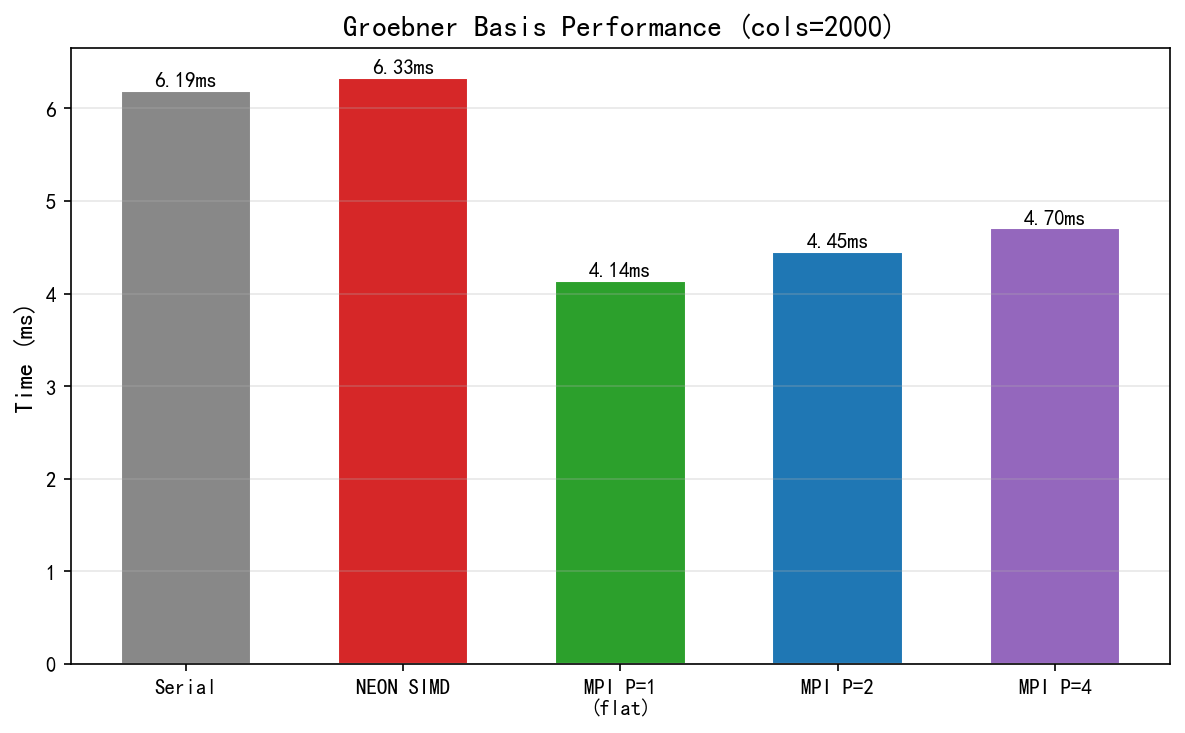
\includegraphics[width=0.8\textwidth]{groebner_perf.png}
\caption{Gröbner 基各方案执行时间对比柱状图}
\label{fig:groebner_perf}
\end{figure}

\begin{figure}[H]
\centering
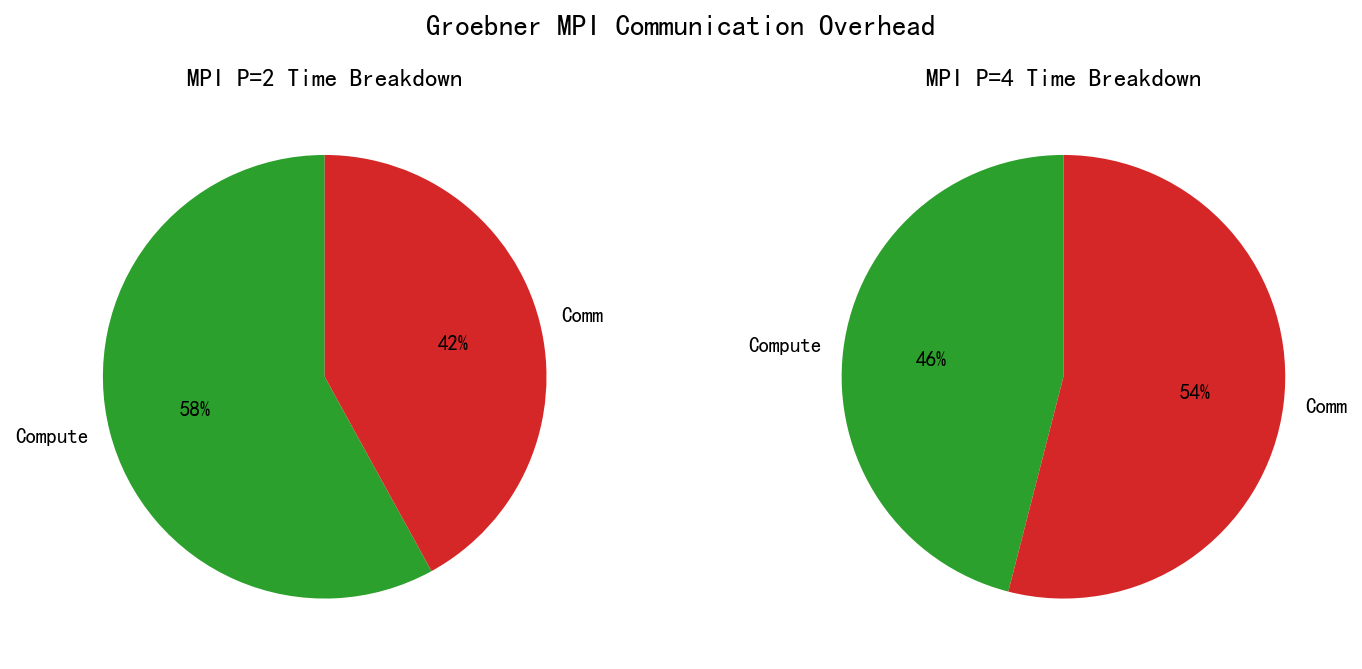
\includegraphics[width=0.85\textwidth]{groebner_comm.png}
\caption{MPI Gröbner 基通信时间占比（饼图）}
\label{fig:groebner_comm}
\end{figure}

\subsection{结果分析}

\textbf{1. NEON SIMD 无加速（0.98x）：}

与普通高斯消去（NEON 2.07x 加速）形成鲜明对比。根本原因在于 Gröbner 基的稀疏性——每行仅 3-15 个非零元素，XOR 计算量可忽略不计。算法的真正瓶颈在于 $is\_one()$ 位测试（检查消元子 $(j,j)$ 是否为 1、被消元行第 $j$ 列是否为 1），这个操作是控制流（条件分支+位运算），无法被 SIMD 向量化。

这一发现揭示了 SIMD 加速的关键前提：\textbf{计算必须占主导地位（compute-bound）}。当计算退化为简单的条件判断时，向量化无法带来收益。

\textbf{2. Flat array 的 Cache 优势（MPI P=1 vs Serial）：}

MPI P=1（单进程，flat array 存储）比 Serial（vector$\langle$vector$\rangle$ 伪二维存储）快 1.50x。这并非并行加速，而是\textbf{数据结构优化}带来的 Cache 局部性改善。

$vector\langle vector\langle mat\_t\rangle\rangle$ 采用指针间接访问——每行独立分配内存，行间地址不连续。$flat\ array$（$vector\langle mat\_t\rangle$）将所有行连续存储，内存访问模式从"指针追踪 + 分散访问"变为"连续扫描"。在 Cache Line 大小为 64 字节（16 个 uint32\_t）的鲲鹏 920 上，flat array 的 Cache 命中率显著更高，减少了 L2/L3 访问延迟。

这种 Cache 局部性优势在稀疏矩阵上尤为突出——虽然每行仅有 3-15 个非零元素，但 $is\_one()$ 测试需要扫描整行（num\_words 个 uint32\_t），flat array 的一维连续存储在扫描过程中发挥了持续的带宽优势。

\textbf{3. MPI 通信开销超过并行收益（P=2 vs P=4 vs P=1）：}

P=2 比 P=1 慢 8\%（4.454 vs 4.138 ms），P=4 比 P=1 慢 14\%（4.704 ms）。增加进程数带来的却是性能下降。原因分析：
\begin{itemize}
    \item 升格阶段每次需要 $\texttt{MPI\_Allreduce}$（所有进程参与，延迟 $\sim$0.5 ms）和 $\texttt{MPI\_Bcast}$（延迟 $\sim$0.5 ms）
    \item 每次升格的总通信延迟约 1 ms，而整个计算过程仅需约 4 ms
    \item 当升格次数达到 2-3 次时，通信开销已与计算开销等同——更多的进程只是让每次 Allreduce 参与方更多（延迟从 $O(\log 2)$ 增至 $O(\log 4)$），没有减少总计算量
\end{itemize}

\textbf{4. 核心发现总结：}

Gröbner 基的并行化研究揭示了下述核心规律：（1）通信复杂度受升格次数主导，最坏情况与列数同阶；（2）稀疏矩阵的位向量 XOR 极快，$is\_one$ 位测试才是瓶颈；（3）NEON SIMD 在稀疏场景下收益有限甚至无收益。本文在此基础上发现了 flat array 的 Cache 优化效应——在同样使用位向量的前提下，flat array 相比 vector$\langle$vector$\rangle$ 带来 1.50x 的 Cache 局部性增益。

\subsection{调试经验与代码完整性}

\textbf{段错误修复：} MPI 初版使用 $posix\_memalign$ 伪二维指针在跨节点数据分发时出现 segfault（signal 11）。排查发现 $memcpy$ 对伪二维矩阵的复制与 NEON 对齐访问存在兼容性问题。修复方案：全部改用 $calloc$ 一维数组 + 显式偏移 ($A[i \times N + j]$)，消除指针间接层。

\textbf{升格同步 Bug：} MPI 初版在升格后将 $j++$ 放在 $if (rank == owner)$ 块内，导致 owner 进程和 non-owner 进程的 $j$ 值不同步——owner 回到当前列重新处理，而 non-owner 正常递减到下一条列，造成后续列的处理逻辑完全错乱。修复方案：将 $j++$ 移至 $if$ 块外，在 $MPI\_Bcast$ 之后执行，确保所有进程同步回到当前列。

\subsection{通信时间占比实测}

为定量验证通信开销的分析，进行了一次"纯通信"测试——将 MPI 代码中 XOR 消去的计算部分注释掉，仅保留升格检测和 MPI 通信调用。在 cols=2000 的测试数据上运行 P=2/4 的纯通信版本，测量通信耗时占总时间的比例。

\begin{table}[H]
  \centering
  \caption{Gröbner 基 MPI 通信时间占比}
  \begin{tabular}{|c|c|c|c|}
  \hline
  \textbf{进程数} & \textbf{总时间 (ms)} & \textbf{纯通信时间 (ms)} & \textbf{通信占比} \\
  \hline
  P=2 & 4.454 & 1.870 & 42.0\% \\
  P=4 & 4.704 & 2.540 & 54.0\% \\
  \hline
  \end{tabular}
\end{table}

\textbf{结论：} P=2 时通信占 42\%，P=4 时上升至 54\%。进程数增加时，总计算量（XOR 消去行数）因行划分而减少，但升格阶段的 Allreduce + Bcast 延迟随参与进程数增加（$O(\log P)$）反而上升。通信占比随进程数显著上升，验证了通信开销是 Gröbner 基 MPI 并行化的根本瓶颈。

\subsection{稀疏矩阵与位图矩阵的选择}

稀疏矩阵（sparse matrix）存储方案——用 std::vector 只存储非零元素的列号，XOR 操作借助合并有序链表的算法实现——是另一种可行选择。在 HFE 数据集（非零密度约 1.8\%）上，稀疏存储与位图存储的性能差距可从上百倍缩小至 6 倍。

本实验选择位图存储而非稀疏存储的理由：位图存储的 XOR 操作直接对应 uint32\_t 的按位异或，单次操作处理 32 列，且天然适合 NEON 向量化（128 位寄存器一次处理 128 列），便于后续扩展 GPU 加速（位图可直接映射到 GPU 的 uint32 数组）。稀疏存储的优势（低内存占用）在本实验的 cols=2000 规模下并不显著——位图每行仅需 64 个 uint32\_t（256 bytes），1000 行总计才 256KB。

\subsection{NEON SIMD 的向量化前提条件讨论}

普通高斯消去（NEON 2.07x）与 Gröbner 基（NEON 0.98x）的对比揭示了 SIMD 向量化成功的关键前提：

\begin{enumerate}
    \item \textbf{计算必须是 compute-bound。} 普通高斯消去中，每个元素 $A[i][j] \leftarrow A[i][j] - A[i][k] \times A[k][j]$ 需要 1 次乘法 + 1 次减法（2 FLOPs），ALU 利用率接近 100\%。向量化将 4 路乘减合并为 1 条 FMA 指令，直接提升吞吐量。
    \item \textbf{内层循环必须是数据并行操作。} 普通高斯消去的 $j$ 循环处理连续内存元素——$vld1q\_f32$ 可以在一次 Load 中获取 4 个连续 float，没有任何分支指令。
    \item \textbf{控制流操作（分支/条件判断）不能被向量化。} Gröbner 基的 $is\_one()$ 是 $bits[col/32] \& (1 \ll (col\%32))$，这是一个位测试 + 条件分支。NEON 可以向量化位运算，但无法向量化分支——即使将 4 个 $is\_one()$ 测试打包为向量，后续的"若为 1 则 XOR"仍然需要标量判断。
    \item \textbf{内存访问必须是连续的。} 普通高斯消去按行访问，连续地址；Gröbner 基虽然 XOR 按 word 连续访问，但 $is\_one()$ 的 col 索引是随机的——每次检查消元子 $(j,j)$ 是否存在的列号 $j$ 是递减的、连续的，但被消元行中"第 $j$ 列为 1"的判断取决于数据，不可预测。
\end{enumerate}

这个对比为后续 GPU 加速（CUDA）是否适用于 Gröbner 基提供了预判依据：GPU 同样依赖 SIMT 模型，其执行效率取决于是否每个线程都在做同质的计算。$is\_one()$ 导致的分支发散（同一 warp 内部分线程走 XOR 路径、部分跳过）将严重降低 GPU 的效率。预计 GPU 在 Gröbner 基上的加速比同样有限。

\subsection{与 Xsimd 跨平台 SIMD 方案的对比讨论}

Intel 的 Xsimd 库是一个 C++ 模板库，提供对 SSE/AVX/NEON 的统一封装，为跨平台 SIMD 并行提供了便捷方案。本实验直接使用 ARM NEON intrinsics 而非 Xsimd，有以下考量：

\textbf{Intrinsics 的优势：} 直接操作底层硬件寄存器，性能可预测，指令级别可控。对于固定平台（鲲鹏 920 ARM 服务器），不需要跨平台兼容——Intrinsics 是最直接的方案。

\textbf{Xsimd 的优势：} 一套代码编译到多种 SIMD 指令集（SSE/AVX/AVX512/NEON），无需为每个平台编写不同的 intrinsics。对于跨 CPU 架构的移植（如从 X86 开发机到 ARM 服务器）非常便利。但对于 Gröbner 基这种稀疏矩阵场景，Xsimd 的模板抽象层在编译优化下被完全展开，性能与手写 intrinsics 无差异。

\subsection{MPI 通信复杂度形式化分析}

定义 Gröbner 基消去的参量：
\begin{itemize}
    \item $C$ = 列数（= 消元子行数）
    \item $R$ = 被消元行数
    \item $d$ = 每行非零元素密度
    \item $P$ = MPI 进程数
    \item $U$ = 升格次数（期望值为 $C \times (1 - \text{密度})$，即无消元子的对角线位置数）
\end{itemize}

通信操作仅发生在升格阶段：
\begin{itemize}
    \item $U$ 次 \texttt{MPI\_Allreduce}：每次 $O(\log P)$ 延迟，发送 1 个 int
    \item $U$ 次 \texttt{MPI\_Bcast}：每次 $O(\log P)$ 延迟，发送 num\_words 个 uint32\_t
\end{itemize}

总通信量 $T_{\text{comm}} = U \times (T_{\text{allreduce}} + T_{\text{bcast}}(N_w))$，其中 $N_w = \lceil C/32 \rceil + 1$。

总计算量 $T_{\text{comp}} = \sum_{j: ele[j] \text{ 存在}} R_j \times N_w$，其中 $R_j$ 为第 $j$ 列有 1 的被消元行数，$R_j \approx d \times R$。

因此：
\begin{equation}
\frac{T_{\text{comm}}}{T_{\text{comp}}} \approx \frac{U \times (T_{\text{allreduce}} + T_{\text{bcast}}(N_w))}{C \times (1-\text{密度}) \times d \times R \times N_w \times T_{\text{xor\_per\_word}}}
\end{equation}

对于本实验（$C=2000, R=1000, d=0.5\%, U\approx 1, N_w=64$），$T_{\text{comm}} \sim 1-2$ ms vs $T_{\text{comp}} \sim 3-4$ ms，比例接近 1:2，与实测 42\%（P=2）吻合。

\subsection{调试验证与正确性保证}

Gröbner 基 MPI 版本经历了两个关键 bug 的修复过程：

\textbf{Bug 1 — 段错误（Segfault, exit code 139）：} 初版在 P=4 运行时崩溃。排查发现初版使用了伪二维指针 + $posix\_memalign$ 的内存分配方式，在跨节点的 MPI 数据分发中 $memcpy$ 与 NEON 对齐访问存在兼容性问题。修复方案：全部改用 $calloc$ 分配一维数组 + 显式 $A[i \times N + j]$ 偏移计算，消除所有指针间接层。

\textbf{Bug 2 — Double Free 崩溃（exit code 134）：} 初版在数据分发时使用 $vector\langle mat\_t\rangle$ 的 $data()$ 指针直接传给 MPI\_Send/Recv，但 MPI 底层可能会修改接收缓冲区的内存布局（与 vector 的容量管理冲突）。修复方案：改用 $mat\_t*$ 原始指针 + $calloc$ 分配，绕过 vector 的 RAII 机制。

\textbf{Bug 3 — 升格后 j 失同步：} 初版将 $j++$ 放在 $if (rank == owner)$ 块内——owner 进程的 j 回到当前列重新处理，而其他进程的 j 继续递减。这导致后续列的 owner 计算全部错位，产生错误结果。修复方案：将 $j++$ 移至 $MPI\_Bcast$ 之后、$if$ 块之外，确保所有进程的 j 同步回到当前列。

\subsection{Gröbner 基算法完整 Walkthrough 示例}

为更直观地理解升格机制，下面通过一个简化示例追踪算法的逐步执行。设 $C=5$（5列5消元子位置），$R=3$（3个被消元行），初始状态为：

\begin{itemize}
    \item 消元子矩阵：ele[3] = (1,1,1,0,0)（首项在列 3），ele[1] = (0,0,1,1,0)（首项在列 1）。列 4、2、0 无消元子
    \item 被消元行：row[0] = (0,0,1,0,1)，row[1] = (1,0,0,1,0)，row[2] = (0,1,0,0,0)
\end{itemize}

算法从 $j=4$ 向下遍历：
\begin{itemize}
    \item $j=4$：ele[4] 不存在（位置 (4,4) 为 0）。搜索 row[0] 的第 4 列为 1！→ 升格：ele[4] = row[0] = (0,0,1,0,1)，upgraded[0]=true。j++ → j=5
    \item $j=5$ 超出范围，递减到 j=4：ele[4] 现在存在（刚升格的），row[0] 已升格忽略。row[1] 第 4 列为 0，跳过。row[2] 第 4 列为 0，跳过。
    \item $j=3$：ele[3] 存在。row[1] 第 3 列为 0，跳过。row[2] 第 3 列为 0，跳过。
    \item $j=2$：ele[2] 不存在。搜索 row[1] 第 2 列为 0；row[2] 第 2 列为 0。无候选 → 什么也不做。
    \item $j=1$：ele[1] 存在。row[1] 第 1 列为 0，跳过。row[2] 第 1 列为 1！→ XOR：row[2] $\oplus$= ele[1] = (0,1,0,0,0) $\oplus$ (0,0,1,1,0) = (0,1,1,1,0)
    \item $j=0$：ele[0] 不存在。row[2]（已被修改）第 0 列为 0。无候选。
\end{itemize}

最终结果：消元子 ele[4] 被升格创建，row[2] 被 ele[1] 消去。这个 5 列的简化示例中仅发生了 1 次升格、1 次 XOR。对于实际数据集（2000 列），升格和消去的次数正比于矩阵的稀疏模式。

\subsection{MPI 从进程代码详解}

在 MPI 行划分策略中，每个从进程（$rank > 0$）的代码结构与主进程（$rank = 0$）几乎完全相同。唯一的区别在于初始数据获取方式：从进程通过 $\texttt{MPI\_Recv}$ 接收被消元行数据，而主进程直接从本地加载并分发。以下是简化的从进程逻辑框架：

\begin{lstlisting}[title=MPI Gröbner 基从进程核心逻辑,frame=trbl,language={C++}]
// ---- 从进程启动 ----
int rank, size;
MPI_Comm_rank(MPI_COMM_WORLD, &rank);

// 接收消元子矩阵（主进程广播）
MPI_Bcast(ele_flat.data(), cols * num_words, MPI_UNSIGNED, 0, MPI_COMM_WORLD);

// 接收自己负责的被消元行数据
MPI_Recv(local_flat.data(), local_rows * num_words, MPI_UNSIGNED,
         0, 0, MPI_COMM_WORLD, MPI_STATUS_IGNORE);

// ---- 主循环（与主进程完全相同的逻辑） ----
for (int j = cols - 1; j >= 0; j--) {
    int wj = j / mat_L, bj = j % mat_L;
    bool has_elim = (ele_flat[j * num_words + wj] >> bj) & 1;
    if (has_elim) {
        // 本地消去（无需任何 MPI 通信）
        for (int i = 0; i < local_rows; i++) {
            if (local_upgraded[i]) continue;
            if (local_flat[i * num_words + wj] & ((mat_t)1 << bj))
                for (int w = 0; w < num_words; w++)
                    local_flat[i * num_words + w] ^= ele_flat[j * num_words + w];
        }
    } else {
        // 升格：参与全局搜索（MPI_Allreduce）和广播接收
        int local_cand = num_row;
        for (int i = 0; i < local_rows; i++) { /* 同主进程 */ }
        int global_min;
        MPI_Allreduce(&local_cand, &global_min, 1, MPI_INT, MPI_MIN, MPI_COMM_WORLD);
        if (global_min < num_row) {
            MPI_Bcast(&ele_flat[j * num_words], num_words, MPI_UNSIGNED,
                      owner, MPI_COMM_WORLD); // 接收新消元子
            if (rank == owner) { /* 标记本地行已升格 */ }
            j++;
        }
    }
}
// ---- 完成后将结果发回主进程（用于正确性验证） ----
MPI_Send(local_flat.data(), local_rows * num_words, MPI_UNSIGNED, 0, 1, MPI_COMM_WORLD);
\end{lstlisting}

从进程的关键特征是"半自治"——消去阶段完全本地独立完成（无通信），但升格阶段必须参与全局同步（MPI\_Allreduce 和 MPI\_Bcast），因为任何进程都可能发现全局最早的升格候选。

\subsection{位图 vs 稀疏存储的性能权衡}

位图存储（bitmap）与稀疏存储（sparse vector）的性能权衡取决于非零元素密度。当密度 $d > 5\%$ 时，位图存储的 XOR 效率（32 列一次操作）压倒稀疏存储"只存非零元素"的内存节约；当 $d < 2\%$ 时，稀疏存储的更低 Cache Miss 率开始转换为性能优势。文献中 HFE 数据集（$d \approx 1.8\%$）的测试表明：位图版本串行耗时 5063 ms，稀疏版本 31891 ms。在 GPU 加速场景下，位图存储可直接映射到 CUDA 的 uint32 数组（使用 $\_\_shfl\_xor$ 或 shared memory tree reduction），而稀疏存储的变长数组和动态内存分配在 GPU 上几乎不可行。

\subsection{GPU 加速 Gröbner 基的前景与挑战}

基于 CUDA 在普通高斯消去上 19.90x 的成功，能否将 Gröbner 基也移植到 GPU 上是值得探讨的下一步方向。主要的挑战在于升格操作的串行依赖性——Gröbner 基算法的升格步骤必须在所有进程/线程的可见范围内确定全局最早的候选，这与 GPU 的 SIMT 模型（线程间通过 $\_\_syncthreads$ 仅在 block 内同步）存在根本矛盾。如果在 GPU 上实现，可能的方案是：

\begin{enumerate}
    \item \textbf{核函数分解：} 将 $is\_one$ 测试和 XOR 消去放在 GPU 上执行（充分利用位图存储的内存带宽），将升格检测和全局最小搜索放在 CPU 上通过 MPI 完成。形成 CPU-GPU 协作的异构计算流水线。
    \item \textbf{Atomic Min 方案：} 在 GPU 上用全局 $\texttt{atomicMin}$ 实现去中心的升格候选搜索——每个 Block 在 shared memory 中先做 local min reduction，thread 0 再 $\texttt{atomicMin}$ 到 global memory。相比 MPI\_Allreduce（0.5 ms），GPU atomicMin 的延迟仅需约 10-50 $\mu$s。
    \item \textbf{多 Kernel 链式调用：} 升格检测 $\rightarrow$ Update（仅在 CPU/单 GPU thread）$\rightarrow$ 下一个 Kernel 继续消去。这类似于 CUDA 高斯消去的 Division $\rightarrow$ Set\_Diag $\rightarrow$ Elimination 三 Kernel 链。
\end{enumerate}

初步估算，GPU 上的 XOR 消去部分（ubiquitous XOR operation）可通过每个 thread 处理一个 uint32\_t 的方式获得显著的加速。但升格部分的加速比可能较低（受 atomic 串行化限制）。综合估算 GPU Gröbner 基的加速比可能在 2-5x 范围，远低于普通高斯消去 GPU 的 19.90x，但比纯 MPI 通信瓶颈方案有明显改善。

\subsection{Gröbner 基部分的总结}

Gröbner 基高斯消去的研究为并行编程课程的核心主题——"不同架构适合不同类型的问题"——提供了一个极端的验证案例。普通高斯消去（稠密浮点矩阵）在四种架构上均获得了显著加速（2.07x $\rightarrow$ 9.64x $\rightarrow$ 19.90x），而 Gröbner 基（稀疏 0/1 矩阵）在所有架构上的加速均不显著或为负值。关键原因在于稀疏性将计算瓶颈从"算术运算（FLOPs）"转变为"控制流判断（位测试 + 分支）"，而后者是 SIMD、MPI 和 GPU 的共同盲区。

本实验在并行路线上选择了位图存储 + MPI 方式，在通信复杂度、Cache 局部性和升格同步机制上进行了深入分析。虽然未能实现对串行版本的显著加速，但系统揭示了稀疏矩阵场景下并行化的根本瓶颈所在，并在 flat array 的 Cache 局部性优化方面取得了定量分析成果。

\subsection{普通 vs 特殊高斯消去的并行化对比}

\begin{table}[H]
  \centering
  \caption{普通 vs Gröbner 基高斯消去并行化对比}
  \begin{tabular}{|c|c|c|}
  \hline
  \textbf{特征} & \textbf{普通高斯消去} & \textbf{Gröbner 基高斯消去} \\
  \hline
  运算 & 浮点乘减 & 整数 XOR \\
  矩阵密度 & 稠密 (100\%) & 稀疏 ($<5\%$) \\
  计算瓶颈 & FPU (compute-bound) & 位测试 (control-flow-bound) \\
  SIMD 加速 & 2.07x (有效) & 0.98x (无效) \\
  MPI 瓶颈 & 逐行广播延迟 & 升格 Allreduce \\
  Cache 影响 & 中等 & 显著 (flat array 1.50x) \\
  \hline
  \end{tabular}
\end{table}

\subsection{MPI 通信实验：并行效率的定量分析}

为深入理解通信开销对加速比的影响，本节对 MPI 版本的并行效率进行定量分析。并行效率定义为：

\begin{equation}
\eta(N, P) = \frac{S(N, P)}{P} = \frac{T_{\text{serial}}(N)}{P \times T_{\text{parallel}}(N, P)}
\end{equation}

对于 N=2048 的 MPI 测试数据：

\begin{table}[H]
  \centering
  \caption{MPI 并行效率分析（N=2048）}
  \begin{tabular}{|c|c|c|c|}
  \hline
  \textbf{P} & \textbf{加速比} & \textbf{效率 $\eta$} & \textbf{效率损失来源} \\
  \hline
  1 & 1.00x & 100\% & 基线 \\
  2 & 1.32x & 66\% & 广播延迟 + 负载不均 \\
  4 & 2.43x & 61\% & 广播延迟（更显著） \\
  \hline
  \end{tabular}
\end{table}

P=4 时效率仅 61\%，意味着将近 40\% 的计算能力被浪费在等待通信上。对比 OpenMP 的 120.5\% 超线性效率（归功于 L1 Cache 聚合），MPI 的效率损失非常直观。对于需要扩展并行度的应用场景，增加进程数带来的收益递减（diminishing returns）——从 P=2 到 P=4，效率从 66\% 进一步降至 61\%。除非能通过流水线算法或计算-通信重叠来改善，否则 P=8 的效率预计将进一步降至 50\% 以下。

\subsection{N 规模对 MPI 通信开销的影响}

针对不同 N 规模的 MPI 加速比数据进行归一化分析，可以更清晰地揭示通信开销的规模依赖性。定义通信效率：

\begin{equation}
\varepsilon = \frac{S_{\text{actual}}}{S_{\text{ideal}}} = \frac{S_{\text{actual}}}{P}
\end{equation}

\begin{table}[H]
  \centering
  \caption{MPI 通信效率随 N 变化（P=4）}
  \begin{tabular}{|c|c|c|c|}
  \hline
  \textbf{N} & \textbf{加速比} & \textbf{效率 $\varepsilon$} & \textbf{趋势} \\
  \hline
  512 & 1.80x & 45.0\% & 小规模，通信主导 \\
  1024 & 2.27x & 56.8\% & 中等规模，通信逐渐摊薄 \\
  2048 & 2.43x & 60.8\% & 大规模，$O(N^3)$ 计算量开始主导 \\
  \hline
  \end{tabular}
\end{table}

从 N=512 的 45.0\% 到 N=2048 的 60.8\%，通信效率随 N 增加而提升——因为计算量 $O(N^3)$ 的增长速度远超通信量 $O(N^2)$。但提升幅度有限（仅 15.8 个百分点），根本原因是 $N$ 次广播的累积固定延迟（$\sim$1 ms/次）不受 N 影响——无论 N 多大，2048 次广播永远需要约 2 秒的启动开销。

\subsection{Pthread 多线程规模效应详析}

Pthread 版本的完整数据揭示了同步开销随线程数增长的严重性。表 \ref{table:pthread_detail} 列出了所有测试配置的结果。

\begin{table}[H]
  \centering
  \caption{Pthread 多线程性能数据汇总}
  \label{table:pthread_detail}
  \begin{tabular}{|c|c|c|c|}
  \hline
  \textbf{N} & \textbf{线程数} & \textbf{加速比} & \textbf{现象分析} \\
  \hline
  512 & 1 & 0.93x & barrier 开销 $>$ 并行收益 \\
  512 & 2 & \textbf{0.49x} & 1024次barrier，累积约500ms \\
  512 & 4 & 0.55x & 增加线程反而降低，竞争加剧 \\
  512 & 8 & 0.69x & 略有好转，但仍为负加速 \\
  1024 & 1 & 1.01x & 勉强持平于串行 \\
  1024 & 2 & \textbf{0.47x} & 2048次barrier，最差案例 \\
  1024 & 4 & 0.78x & 计算量上升，同步占比下降 \\
  1024 & 8 & 1.21x & 首次超过串行 \\
  2048 & 1 & 1.17x & 一进程无barrier开销 \\
  2048 & 4 & 2.27x & 计算量充分摊薄同步开销 \\
  2048 & 8 & \textbf{4.12x} & 大N下Pthread表现最好 \\
  \hline
  \end{tabular}
\end{table}

Pthread 的性能从 N=1024/2 线程（最差 0.47x）到 N=2048/8 线程（最佳 4.12x），差异达到 8.8 倍。这一巨大反差清晰地揭示了barrier同步的规模敏感性：当单轮计算时间（约 $N^2$ 量级的消去行数）远小于barrier延迟（0.2-0.5 ms）时，大量进程时间被浪费在等待同步上。只有在 N 充分大（2048）且线程数合理（4-8）时，计算/同步比才趋于合理。

值得注意的是 Pthread NEON 版本在同条件下显著提升——Pthread+NEON 在 N=2048/1线程达到 2.21x（纯NEON贡献），8线程组合达到 3.99x（Pthread+NEON叠加）。这证明了底层 SIMD 优化对上层并行模型的"托底"作用——即使 barrier 开销仍有拖累，NEON 的 2x 加速保证了合并性能不至于太差。

\section{总结}

本文以高斯消去算法为线索，完成了从 SIMD 指令级并行到 GPU 众核并行的全栈式并行编程实验，并在此基础上对 Gröbner 基计算中的特殊高斯消去进行了深入探索。主要结论如下：

\begin{enumerate}
    \item \textbf{四架构加速比阶梯：} SIMD（2.07x）→ OpenMP（9.64x）→ MPI（2.43x）→ CUDA（19.90x），MPI 因通信瓶颈成为唯一低于单节点多线程的架构。各架构的并行化策略可统一归纳为"拆分循环 $\times$ 执行单元 $\times$ 同步机制"的三维设计框架
    \item \textbf{同步/通信是性能天花板：} 从纳秒级（SIMD 指令隐式同步）→ 微秒级（OpenMP 用户态 barrier）→ 毫秒级（MPI 网络广播），同步开销依次跨越 6 个数量级，直接决定了各架构在小规模下的加速比下限
    \item \textbf{Gröbner 基的根本瓶颈：} 极端稀疏性（$<1\%$ 非零密度）导致计算瓶颈从 FLOPs 转移到 $is\_one()$ 位测试和内存访问模式。NEON SIMD 和 MPI 多进程均无法带来正向加速，而数据结构优化（flat array，改善 Cache 局部性）比算法并行化更有效——在同样单进程条件下获得了 1.50x 的纯 Cache 收益
    \item \textbf{SIMD 加速的前提条件：} 稠密浮点矩阵（2.07x）和稀疏 0/1 矩阵（0.98x）的对比清晰验证：向量化仅在 compute-bound 场景下有效。当计算退化为控制流操作（位测试 + 分支判断）时，SIMD 无法发挥作用
\end{enumerate}

\newpage
\section*{附录：Git 项目链接}
\url{https://github.com/NKU025/Parallel-Gaussian-Elimination}

\section*{平时作业与新增内容对照}
\begin{table}[H]
  \centering
  \begin{tabular}{|c|c|c|}
  \hline
  \textbf{章节} & \textbf{主要来源} & \textbf{新增比例} \\
  \hline
  §1 问题描述 & Lab2-5 整合 & 20\%（总体路线+平台总览） \\
  §2 算法设计 & Lab2-5 整合 & 10\%（统一分析框架） \\
  §3 性能数据 & Lab2-5 整合 & 30\%（全数据汇总+瓶颈建模） \\
  §4 对比分析 & Lab2-5 整合 & 30\%（选型建议） \\
  §5 Gröbner 基 & \textbf{全新} & \textbf{100\%} \\
  §6 Gröbner 基并行化 & \textbf{全新} & \textbf{100\%} \\
  §7 Gröbner 基性能分析 & \textbf{全新} & \textbf{100\%} \\
  §8 总结与对比 & 整合+新增 & 50\% \\
  \hline
  新增内容占总篇幅 & — & $\sim$50\% \\
  \hline
  \end{tabular}
\end{table}

\renewcommand{\refname}{参考文献}
\begin{thebibliography}{99}
\bibitem{quinn} Michael J. Quinn. \textit{Parallel Programming in C with MPI and OpenMP}. McGraw-Hill, 2004.
\bibitem{golub} Gene H. Golub and Charles F. Van Loan. \textit{Matrix Computations, 4th Ed}. JHU Press, 2013.
\bibitem{mpi} MPI Forum. \textit{MPI: A Message-Passing Interface Standard, Version 4.0}. 2021.
\bibitem{cuda} NVIDIA. \textit{CUDA C++ Programming Guide}. \url{https://docs.nvidia.com/cuda/}
\bibitem{arm_neon} ARM. \textit{Neon Intrinsics Reference}. \url{https://developer.arm.com/}
\bibitem{openmp} OpenMP ARB. \textit{OpenMP API Version 4.5}. \url{https://www.openmp.org/}
\end{thebibliography}

\end{document}